\documentclass{article}

\usepackage{hyperref}
\hypersetup{
	colorlinks=true,
	linkcolor=blue,
	urlcolor=cyan,}
\usepackage{booktabs}
\usepackage{textgreek}

%%%%%%%%%%%%%%%%%%%%%%%%%%%%%%%%%%%%%%%%%
% Lachaise Assignment
% Structure Specification File
% Version 1.0 (26/6/2018)
%
% This template originates from:
% http://www.LaTeXTemplates.com
%
% Authors:
% Marion Lachaise & François Févotte
% Vel (vel@LaTeXTemplates.com)
%
% License:
% CC BY-NC-SA 3.0 (http://creativecommons.org/licenses/by-nc-sa/3.0/)
% 
%%%%%%%%%%%%%%%%%%%%%%%%%%%%%%%%%%%%%%%%%

%----------------------------------------------------------------------------------------
%	PACKAGES AND OTHER DOCUMENT CONFIGURATIONS
%----------------------------------------------------------------------------------------

\usepackage{amsmath,amsfonts,stmaryrd,amssymb} % Math packages

\usepackage{enumerate} % Custom item numbers for enumerations

\usepackage[ruled]{algorithm2e} % Algorithms

\usepackage[framemethod=tikz]{mdframed} % Allows defining custom boxed/framed environments

\usepackage{listings} % File listings, with syntax highlighting
\lstset{
	basicstyle=\ttfamily, % Typeset listings in monospace font
}

%----------------------------------------------------------------------------------------
%	DOCUMENT MARGINS
%----------------------------------------------------------------------------------------

\usepackage{geometry} % Required for adjusting page dimensions and margins

\geometry{
	paper=a4paper, % Paper size, change to letterpaper for US letter size
	top=2.5cm, % Top margin
	bottom=3cm, % Bottom margin
	left=2.5cm, % Left margin
	right=2.5cm, % Right margin
	headheight=14pt, % Header height
	footskip=1.5cm, % Space from the bottom margin to the baseline of the footer
	headsep=1.2cm, % Space from the top margin to the baseline of the header
	%showframe, % Uncomment to show how the type block is set on the page
}

%----------------------------------------------------------------------------------------
%	FONTS
%----------------------------------------------------------------------------------------

\usepackage[utf8]{inputenc} % Required for inputting international characters
\usepackage[T1]{fontenc} % Output font encoding for international characters

\usepackage{XCharter} % Use the XCharter fonts

%----------------------------------------------------------------------------------------
%	COMMAND LINE ENVIRONMENT
%----------------------------------------------------------------------------------------

% Usage:
% \begin{commandline}
%	\begin{verbatim}
%		$ ls
%		
%		Applications	Desktop	...
%	\end{verbatim}
% \end{commandline}

\mdfdefinestyle{commandline}{
	leftmargin=10pt,
	rightmargin=10pt,
	innerleftmargin=15pt,
	middlelinecolor=black!50!white,
	middlelinewidth=2pt,
	frametitlerule=false,
	backgroundcolor=black!5!white,
	frametitle={Command Line},
	frametitlefont={\normalfont\sffamily\color{white}\hspace{-1em}},
	frametitlebackgroundcolor=black!50!white,
	nobreak,
}

% Define a custom environment for command-line snapshots
\newenvironment{commandline}{
	\medskip
	\begin{mdframed}[style=commandline]
}{
	\end{mdframed}
	\medskip
}

%----------------------------------------------------------------------------------------
%	FILE CONTENTS ENVIRONMENT
%----------------------------------------------------------------------------------------

% Usage:
% \begin{file}[optional filename, defaults to "File"]
%	File contents, for example, with a listings environment
% \end{file}

\mdfdefinestyle{file}{
	innertopmargin=1.6\baselineskip,
	innerbottommargin=0.8\baselineskip,
	topline=false, bottomline=false,
	leftline=false, rightline=false,
	leftmargin=2cm,
	rightmargin=2cm,
	singleextra={%
		\draw[fill=black!10!white](P)++(0,-1.2em)rectangle(P-|O);
		\node[anchor=north west]
		at(P-|O){\ttfamily\mdfilename};
		%
		\def\l{3em}
		\draw(O-|P)++(-\l,0)--++(\l,\l)--(P)--(P-|O)--(O)--cycle;
		\draw(O-|P)++(-\l,0)--++(0,\l)--++(\l,0);
	},
	nobreak,
}

% Define a custom environment for file contents
\newenvironment{file}[1][File]{ % Set the default filename to "File"
	\medskip
	\newcommand{\mdfilename}{#1}
	\begin{mdframed}[style=file]
}{
	\end{mdframed}
	\medskip
}

%----------------------------------------------------------------------------------------
%	NUMBERED QUESTIONS ENVIRONMENT
%----------------------------------------------------------------------------------------

% Usage:
% \begin{question}[optional title]
%	Question contents
% \end{question}

\mdfdefinestyle{question}{
	innertopmargin=1.2\baselineskip,
	innerbottommargin=0.8\baselineskip,
	roundcorner=5pt,
	nobreak,
	singleextra={%
		\draw(P-|O)node[xshift=1em,anchor=west,fill=white,draw,rounded corners=5pt]{%
		Question \theQuestion\questionTitle};
	},
}

\newcounter{Question} % Stores the current question number that gets iterated with each new question

% Define a custom environment for numbered questions
\newenvironment{question}[1][\unskip]{
	\bigskip
	\stepcounter{Question}
	\newcommand{\questionTitle}{~#1}
	\begin{mdframed}[style=question]
}{
	\end{mdframed}
	\medskip
}

%----------------------------------------------------------------------------------------
%	WARNING TEXT ENVIRONMENT
%----------------------------------------------------------------------------------------

% Usage:
% \begin{warn}[optional title, defaults to "Warning:"]
%	Contents
% \end{warn}

\mdfdefinestyle{warning}{
	topline=false, bottomline=false,
	leftline=false, rightline=false,
	nobreak,
	singleextra={%
		\draw(P-|O)++(-0.5em,0)node(tmp1){};
		\draw(P-|O)++(0.5em,0)node(tmp2){};
		\fill[black,rotate around={45:(P-|O)}](tmp1)rectangle(tmp2);
		\node at(P-|O){\color{white}\scriptsize\bf !};
		\draw[very thick](P-|O)++(0,-1em)--(O);%--(O-|P);
	}
}

% Define a custom environment for warning text
\newenvironment{warn}[1][Warning:]{ % Set the default warning to "Warning:"
	\medskip
	\begin{mdframed}[style=warning]
		\noindent{\textbf{#1}}
}{
	\end{mdframed}
}

%----------------------------------------------------------------------------------------
%	INFORMATION ENVIRONMENT
%----------------------------------------------------------------------------------------

% Usage:
% \begin{info}[optional title, defaults to "Info:"]
% 	contents
% 	\end{info}

\mdfdefinestyle{info}{%
	topline=false, bottomline=false,
	leftline=false, rightline=false,
	nobreak,
	singleextra={%
		\fill[black](P-|O)circle[radius=0.4em];
		\node at(P-|O){\color{white}\scriptsize\bf i};
		\draw[very thick](P-|O)++(0,-0.8em)--(O);%--(O-|P);
	}
}

% Define a custom environment for information
\newenvironment{info}[1][Info:]{ % Set the default title to "Info:"
	\medskip
	\begin{mdframed}[style=info]
		\noindent{\textbf{#1}}
}{
	\end{mdframed}
}
 % Include the file specifying the document structure and custom commands

%----------------------------------------------------------------------------------------
%	ASSIGNMENT INFORMATION
%----------------------------------------------------------------------------------------

\title{OIA Lab 1: Introduction to ELVIS Virtual Instrumentation}
\author{BIOE 385 Bioinstrumentation Laboratory} 
\date{}
%----------------------------------------------------------------------------------------

\begin{document}
\large
\maketitle

\section*{Goals}
\begin{enumerate}
	\item Become familiar with the NI-ELVIS Setup and Virtual Instrumentation
	\item Perform simple analysis of practical DC circuits using ELVIS
	\item Investigate the behavior of an RC circuit
\end{enumerate}

\section*{Textbook Readings}
Note: these readings will help you with your project.  You are responsible for knowing this information before next lab although these should be a review.
\begin{itemize}
	\item 7.1: Safety
	\item 2.1-3: Theory of Electronics, Electric Current and Voltage
	\item 2.9-12: Wire Gauges, Grounds, Electric Circuits, Ohm's Law and Resistors
	\item 2.14: Measuring Voltage, Current and Resistance
	\item 2.16: Open and Short Circuits
\end{itemize}

\section*{Part 1: ELVIS Orientation}
\subsection*{Introduction}

The system you will be working with in the labs for this course is called ELVIS and was developed by \href{www.ni.com}{National Instruments (NI)}. ELVIS stands for Educational Laboratory Virtual Instrumentation Suite. A virtual instrument (VI) is essentially a software representation of a physical instrument. In the study of circuits, we commonly use three instruments – function generators, oscilloscopes and power supplies. The ELVIS system can recreate the functions of these instruments on the computer, thus simplifying our bench setup.\\

The ELVIS system uses software to replicate:
\begin{itemize}
	\item \textbf{A function generator} - an instrument capable of producing periodic voltage waveforms (e.g. sine waves, square waves, triangular waves), at different frequencies and amplitudes. It is used to provide voltage input to test the output response of a circuit.
	\item \textbf{An oscilloscope} - an electronic instrument that graphically displays a measured voltage (y-axis) as a function of time (x-axis). For example, the oscilloscope will be used to display the output from a function generator in part two of this lab.
	\item \textbf{A variable power supply} - an instrument that is used as a source of potential difference for use in circuitry, (e.g. to provide a DC voltage).
	\item \textbf{A digital multi-meter (DMM)} - an instrument that is used to measure two or more electrical values - often times voltage (volts), current (amps) and resistance (ohms).
\end{itemize}

This software can also be used to perform useful functions such as creating a \textbf{bode plot} of the frequency response of a circuit.\\

The first time you run ELVIS you will need to perform a self-calibration. You might also want to do this periodically to improve the accuracy of your system - in order to compensate for inherent sources of error commonly found on electronic components, such as nonlinearities and drift due to time and temperature. 

\subsection*{Getting Started}
The NI ELVIS II Series Prototyping Board (protoboard) connects to the workstation and provides an area for building electronic circuitry.

\begin{warn}
	Always ensure that the prototyping board power switch is off before inserting or removing it from the workstation.
\end{warn}

\begin{enumerate}
	\item Install your \textbf{NI ELVIS Protoboard} on top of the ELVIS II unit – make sure it is properly aligned at the front and back and push until you hear a click. \textit{Tip: use one hand to hold the back of the unit, while you use the other hand to push the protoboard in place.}
		\begin{figure}[h]
    	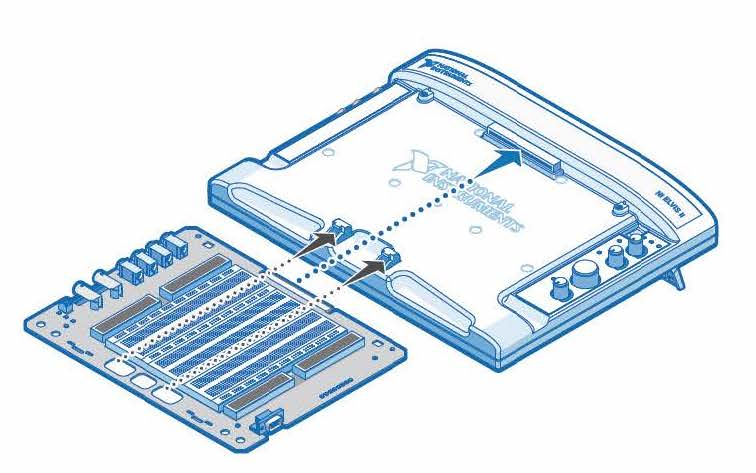
\includegraphics[width=0.5\textwidth]{lab_1_fig_1.jpg}
    	\centering
		\end{figure}
	\item Turn on your ELVIS unit’s system power – this is located on the back panel of the unit. The orange \textbf{USB READY} LED indicator on the front panel should now be lit.
	\item Turn on the prototyping board power switch located on the top of the unit (see diagram). The green \textbf{PROTOTYPING BOARD POWER} LED should now be lit.
		\begin{figure}[h!]
    	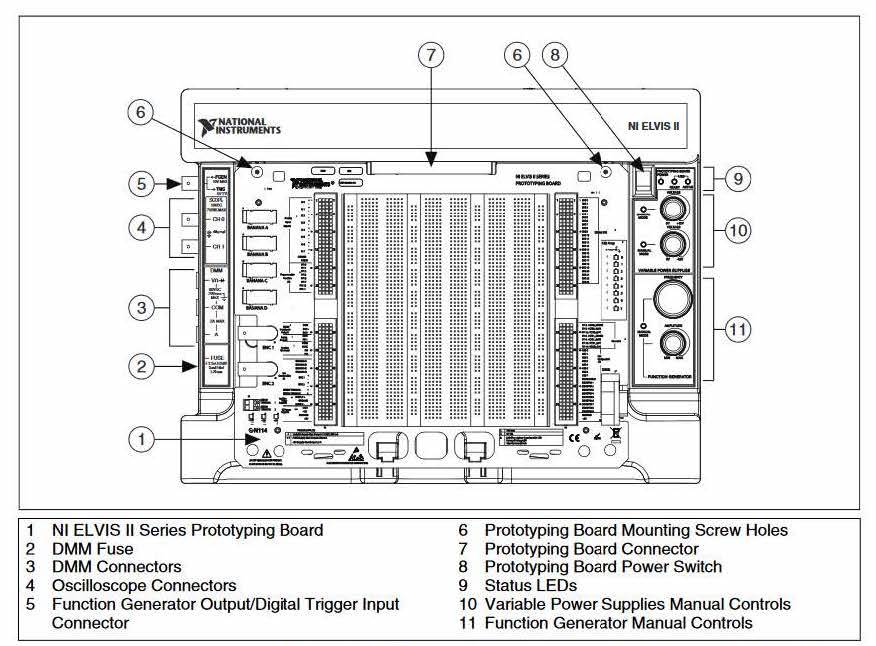
\includegraphics[width=0.8\textwidth]{lab_1_fig_2.jpg}
    	\centering
		\end{figure}
\end{enumerate}

\subsection*{Self-calibration Routine}
Always perform this step with the prototyping board power ON. Step-by-step instructions are as follows:

\begin{enumerate}
	\item Double-click on the NI MAX icon on the desktop. If the icon is not present, follow Start $\rightarrow$ Programs $\rightarrow$ Applications $\rightarrow$ National Instruments $\rightarrow$ NI ELVISmx for NII ELVIS \& NI myDAQ $\rightarrow$ NI ELVISmx Instrument Launcher.
	\item Under Resources, double click Measurement and Automation Explorer.
	\item Expand the My System $\rightarrow$ Devices and Interfaces $\rightarrow$ NI ELVIS II “Dev1”.
	\item Click on NI ELVIS II “Dev1”.
	\item Click on Self Test and wait for the “The self test completed successfully” message.
	\item Next, click on Self-Calibrate and wait for the operation to continue.
	\item Close the Test Panel window and you are ready to continue to the next step.
\end{enumerate}

\subsection*{Introduction to ELVIS}
\begin{enumerate}
	\item Double-click on the NI ELVIS Instrument Launcher icon found on the desktop. If the icon is not present, follow Start $\rightarrow$ Programs $\rightarrow$ Applications $\rightarrow$ National Instruments $\rightarrow$ NI ELVISmx for NI ELVIS \& NI myDAQ $\rightarrow$ NI ELVISmx Instrument Launcher.
	\item From the Instruments \& Apps menu, select the Oscilloscope option. The NI-ELVIS virtual instrument oscilloscope is capable of reading signals from the built-in ELVIS SCOPE (ch0 and ch1) or from circuits on the protoboard (AI 0 thru AI 7).
		\begin{enumerate}
			\item The NI ELVIS oscilloscope can display signals from the Analog Input Channels (AI 0-7) located in your protoboard.
			\item Connect a wire from the function generator output to the analog input channel 0+ and ground the AI0- channel directly using AIGND. Make sure the oscilloscope source is the same channel as the one you are feeding your signal to. \textit{A general safety guideline is to make connections while the prototype board power is off.}
			\item Click Run (you will not see your signal yet; continue to next step).
		\end{enumerate}
	\item From the Instruments \& Apps menu, choose the Function Generator option and click on Manual Mode. Generate a signal using the manual controls (these are found on the ELVIS II unit’s front panel) for the function generator. The manual mode LED should be ON. If you want to control the function generator with the ELVIS software, unclick Manual Mode on your virtual instrument (controlled via computer).
		\begin{enumerate}
			\item Turn on Manual Mode.
			\item On the ELVIS unit’s function generator panel, select the sine wave signal option
			\item Using the knobs on the ELVIS unit, adjust the frequency to 500 Hz, and turn the amplitude to 3/4 of the maximum setting (indicator should be pointing right).
			\item On the oscilloscope screen, notice that you can see the root-mean-squared (RMS) amplitude, frequency, and peak-to-peak amplitude (Vp-p) of the input signal displayed. What exactly do these parameters refer to?
			\item Adjust the oscilloscope vertical scale such that the signal height (peak to peak) covers approximately 2 squares. What is your vertical scale?
			\item Adjust the timebase. What is happening to your signal? Select a value that results in a few cycles of your signal displayed on screen.
		\end{enumerate}
	\item Does your signal appear stable on oscilloscope screen?
	\item Have an instructor or TA check your answers and show them your signal.
\end{enumerate}

\underline{Triggers} are used to stabilize signals viewed using oscilloscopes. They function by ensuring that the horizontal sweep (signal reading) always begins at the same point of a repeating signal, resulting in a clear picture. The most common type of triggering is \underline{edge triggering}, where the sweep begins when the input signal rises or falls past a certain voltage level. The ELVIS system has a built-in function for edge triggering that is synchronized with the signal being generated by the function generator.\\

\begin{enumerate}
	\item Select EDGE for the type on the trigger menu and Chan 0 for your source. What happens to your signal?
	\item You are now looking at your triggered signal. Experiment by adjusting the amplitude and frequency controls on the ELVIS unit. Change the slope, level and horizontal positions. How do these changes affect the triggered signal? Describe how you think the trigger is working.
	\item Select Run Once under Acquisition Mode on the Oscilloscope screen. Describe the difference between this option and using a trigger signal.
	\item Return to Run Continuously and click the Log button to save the data for the sweep as a txt (text) file. Open the file and understand how your data has been recorded.
	\item The previous section used the function generator built into the ELVIS unit. Now generate a signal using the virtual instrument function generator.
		\begin{enumerate}
			\item Open the Function Generator from the ELVIS menu. \textit{At this point, you must switch the manual control of the ELVIS unit function generator off.}
			\item Turn on the virtual instrument function generator and select a triangular waveform with 500 Hz frequency and set the peak amplitude to 2.0 V (4Vpp).
			\item Adjust your oscilloscope display to show 5 cycles starting and ending at the highest point (signal should look like: VVVVV). Each cycle should cover 2 squares vertically and 2 squares horizontally. Write down the values you used to achieve this.
			\item Adjust the DC offset of your signal and describe what happens.
			\item Show your signal (described above) to an instructor or TA.
		\end{enumerate}
\end{enumerate}

\subsection*{Introduction to the ELVIS Prototyping board}
\begin{enumerate}
	\item Identify the 5 individual protoboards within the full ELVIS protoboard. The protoboards on the far left and far right each contain four columns of pin sockets. Each row on these left and right protoboards is connected to the main ELVIS unit or the connectors on the protoboard, to send/receive signals to/from these locations, and are grouped according to their function. For example, locate the group of pin sockets labeled Function Generator (FUNC\_OUT). Within this group, all the rows deliver the same waveform from the function generator (ELVIS unit front panel or virtual instrument), that we previously displayed on the virtual oscilloscope screen. IMPORTANT: All four pin sockets in each row are connected together to the terminal labeled on the protoboard. For example, all four pin sockets in the +5 V row are at a potential of +5 V. All four pin sockets in the GROUND row are at a potential of 0 V.
	\item Locate the rows of four pin sockets at +5 V and Ground. Use a wire to connect one of the +5 V pins to a pin for any one of the group of 8 LEDs (on the right side of your protoboard). Use a second wire to light any other LED from another pin on the +5 V supply. Is it clear how the rows and columns of pin sockets are connected in the left and right protoboards? You should have two LEDs lit.
	\item The three protoboards in the center of the ELVIS unit contain more pin sockets arranged in rows and columns. Using your wires to map out the connections between pins in each of the sections of the protoboard (i.e. connect the 5V DC to socket A60 on your prototyping board and use a different wire to connect your LED to A59. Does the LED light up? What if you connect the LED wire to B60 instead?). Use colored pens or pencils to label/illustrate these connections. Only one or two rows/columns need to be drawn for each section.
\end{enumerate}

\begin{warn}
	If you are confused about any of the concepts introduced so far, ask for clarification from an instructor or TA. We will be using ELVIS every week, so it is critical that you understand the system to \textit{save time in future weeks.} 
\end{warn}

\section*{Part 2: DC Analysis of Simple Circuits}
\subsection*{Introduction}
In this section of the lab, you will use the ELVIS system to analyze the direct current (DC) response of different circuits. The following instructions will suggest methods you can follow in your analysis. You are free to experiment with other options within ELVIS to perform the requested measurements; if in doubt, ask a TA during lab for assistance. For reference, when we say “measure the voltage (or potential) between point A and point B”, we mean “measure the potential \textit{difference} between point A and point B”. If we just say “measure the voltage at point B”, we mean “measure the potential difference between point B and ground” (which we define as 0 volts).

\subsection*{Voltage Divider}
The figure below depicts a voltage divider.
\begin{figure}[h!]
    	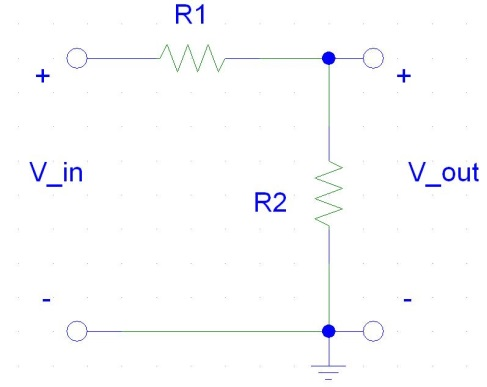
\includegraphics[width=0.4\textwidth]{lab_1_fig_3.jpg}
    	\centering
		\end{figure}

\begin{enumerate}
	\item What is the relationship between the input voltage, V\_in, and the output voltage, V\_out, in terms of R1 and R2?
	\item In general, such relationships between input and output signals are to be referred to as transfer functions, because they describe the transfer of information, in this case a voltage, from the input to the output of a device. We can represent the transfer function, $H$, by the relationship:

		$$V_{out} = H \times V_{in}$$
		
	\item Assume that we want H = 0.5 for the voltage divider. If R2 = 100 \textOmega, what should R1 be?
	\item Construct a voltage divider on the ELVIS protoboard using the values of R1 and R2 from part 3 above. Do not apply V\_IN yet.
	\item Now apply a DC input to the voltage divider (V\_IN), and measure the output (V\_OUT). One way to apply a DC input is to use the virtual instrument function generator from Part 1. To do this, connect a wire to the variable power supply and set it to 2V. This produces a constant output voltage; check this with the virtual oscilloscope. Use a wire to apply this power supply output to your voltage divider at the V\_IN + point. (Recall from the last section how the signals are delivered to the protoboard). Measure the output voltage (the voltage across R2). You can use either the digital oscilloscope included in ELVIS, or the handheld FLUKE multimeters. Ask the TAs about how to use the multimeters.
	\item What output do you expect? What output do you see? \textit{If your output doesn’t quite match what you expected to see, why do you think this is the case? If your output does match what you expect, can you speculate why it wouldn’t? Where are inaccuracies most likely to come from?}
	\item Rearrange your voltage divider to obtain a transfer function H= 0.3. Input a 3Vp-p sinusoidal signal into your voltage divider. Show the TA your results. Describe the results you obtain.
\end{enumerate}

\subsection*{Using a variable resistor (potentiometer)}
Potentiometers provide varying degrees of resistance that can be set by turning a manual knob. The movable element (wiper) makes contact with a resistive strip of material closer to or further away from each one of the two terminals, therefore varying the resistance across. In this section, we will learn how potentiometers work and how to wire them.
\begin{figure}[h!]
    	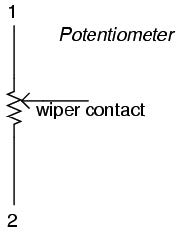
\includegraphics[width=0.3\textwidth]{lab_1_fig_4.jpg}
    	\centering
		\end{figure}
\begin{enumerate}
	\item Using 5VDC as your input, create the following circuit (rheostat) using a 200 W potentiometer. \textit{Note: Ignore the load for now.}
		\begin{figure}[h!]
    	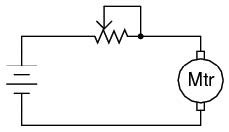
\includegraphics[width=0.3\textwidth]{lab_1_fig_5.jpg}
    	\centering
		\end{figure}
	\item Connect the potentiometer using the middle and one of the side leads (wire the unused terminal to the middle lead or wiper).
	\item Adjust the resistance by turning the screw on the pot.
	\item Using an external DMM to adjust the resistance across the two connected terminals of your potentiometer, and the ELVIS oscilloscope to measure the voltage across your potentiometer, calculate current output across your ‘load.’ Record your findings in the following table. \textit{Note: turn off your protoboard power when measuring the resistance/adjusting the pot.}
		
		\begin{table}[h!]
		\centering
		\begin{tabular}[h!]{c|c|c}
		\toprule
		Resistance (\textOmega) & Voltage across the pot (V) & Current (I) \\
		\midrule
		10 & &\\
		\midrule
		50 & &\\
		\midrule
		100 & &\\
		\midrule
		150 & &\\
		\midrule
		200 & &\\
		\bottomrule
		\end{tabular}
		\end{table}

	\item What would happen if the resistance between your connected terminals is decreased until it reads 0\textOmega?
	\item Explain how this is circuit is working and possible applications of this setup. \textit{Hint: if you are still not sure about what you are seeing, connect an external DMM to measure the current as you adjust your pot.}
\end{enumerate}

\subsection*{Back to Voltage Dividers}
\begin{enumerate}
	\item Using a 5VDC as your input, create the following circuit using a 200\textOmega potentiometer.
 		\begin{figure}[h!]
    	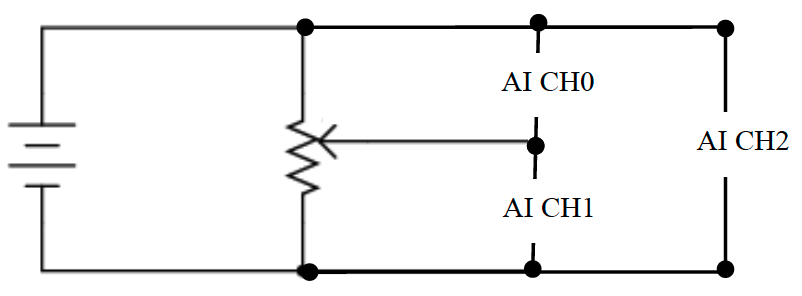
\includegraphics[width=0.6\textwidth]{lab_1_fig_6.png}
    	\centering
		\end{figure}
	\item Connect the potentiometer using all 3 terminals (5V and ground should be connected to the outer terminals).
	\item Adjust the resistance by turning the screw on the pot (measure using and external DMM).
	\item Using the virtual NI ELVIS II oscilloscope, describe the behavior you observe in Ch0, Ch1 and Ch2 as you turn the knob on the potentiometer.
	\item Explain how this is circuit is working and possible applications of this setup.
\end{enumerate}

\subsection*{Wheatstone Bridge}
Modifying the topology of the divider from part I (H=0.5; R2=100\textOmega) and re-labeling “V\_out” as “V\_a”, we have:

\begin{figure}[h!]
    	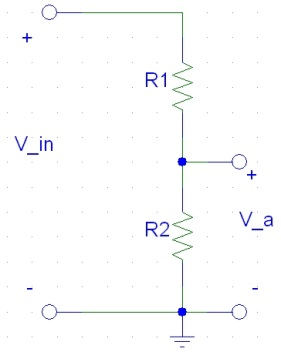
\includegraphics[width=0.3\textwidth]{lab_1_fig_7.jpg}
    	\centering
		\end{figure}

We can add another, identical voltage divider to this circuit (do not build until step 3)\\

\begin{figure}[h!]
    	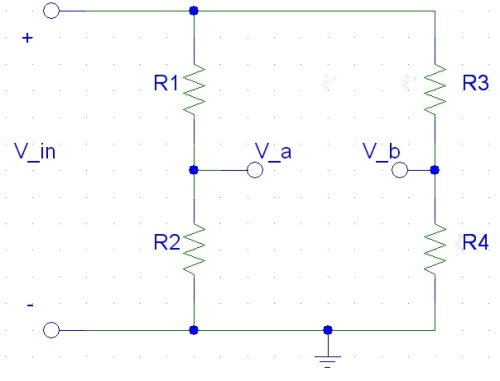
\includegraphics[width=0.5\textwidth]{lab_1_fig_8.jpg}
    	\centering
		\end{figure}

where R1 = R3, and R2 = R4.

\begin{enumerate}
	\item Using the values of R1 and R2 from part (I), what do you expect the value of V\_a to be in terms of V\_in? What about V\_b?
	\item If you consider your output, “V\_out”, to be the difference between V\_a and V\_b, what would you expect this output to be?
	\item Construct the Wheatstone bridge by building off of your circuit from 1. However, use a strain gage instead of R4. Strain gages are wafer like resistors whose resistance changes in response to being stretched or compressed. The gage is a two-terminal device that is mounted onto a surface and allows you to measure strain in the material.
	\item Apply a DC voltage across the V\_in terminals (you can use the same input from part (I), and measure the potential at V\_a. Measure V\_b. Are they the same? If not, why not?
	\item With no strain applied to the gage, we require V\_a = V\_b, which would result in V\_out = 0. i.e. a balanced bridge. This is necessary to be able to accurately detect changes in strain when resistance changes in any one arm of the bridge. To do this, we can substitute a potentiometer and balance the bridge. Replace R2 with a 200\textOmega pot (use rheostat configuration from above). Balance the bridge by measuring V\_out and adjust the pot resistance until V\_out = 0.
	\item Now that you have balanced the bridge, gently bend the material. You don’t want to create a permanent deformation or break it – so please be gentle. What do you see? How does the circuit output vary in response to compression and tension? Qualitatively, how sensitive is the strain gauge?
	\item Use the oscilloscope to record some of your observations (a second or two will suffice).
	\item How does the relative change in resistance of the gage depend on the applied strain? How would the output voltage of the bridge relate to the strain? Why does it make sense to have the baseline V\_out = 0?
\end{enumerate}

\end{document}
